\section{B+树索引文件}

\subsection{B+树索引文件}

B+树索引是索引顺序文件的一种替代方案。

\begin{itemize}
    \item 索引顺序文件的缺点:随着文件增长性能下降,因为会创建许多溢出块;需要定期对整个文件进行重组。
    \item B+树索引文件的优点:面对插入和删除操作时,能通过小规模的局部更改自动进行自我重组;无需对整个文件进行重组即可保持性能。
    \item (次要)B+树的缺点:额外的插入和删除开销;空间开销。
    \item B+树的优点大于缺点:被广泛应用
\end{itemize}

B+树是一种满足以下性质的有根树:

\begin{itemize}
    \item 从根节点到叶节点是所有路径相同---平衡树
    \item 每个非根节点和非叶节点有介于$\lceil n/2 \rceil$到$n$个孩子节点
    \item 叶节点有介于$\lceil (n-1)/2 \rceil$到$n-1$个值
    \item 特殊情况:
       \begin{itemize}
           \item 如果根节点不是叶节点,它至少有2个孩子节点
           \item 如果根节点是叶子节点(即树中没有其它节点),那么它可以有0到$n-1$个值。
       \end{itemize}
\end{itemize}

\subsection{B+树节点结构}

3种典型节点:

\begin{figure}[H]
    \centering
    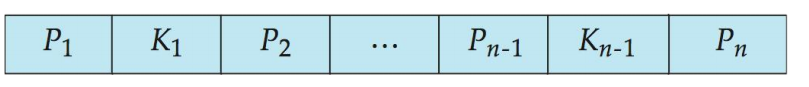
\includegraphics[width=0.9\linewidth]{image5.png}
    \caption{B+树节点}
    \label{}
\end{figure}

\begin{itemize}
    \item $K_i$是搜索键值
    \item $P_i$是指向子节点的指针(对于非叶节点)或指向记录或记录桶的指针(对于叶节点)
    \item 通常,一个节点对应一个block
\end{itemize}

节点中的搜索键是有序的:
$$K_1<K_2<...<K_{n-1}$$
(最初假设没有重复键,稍后处理重复问题)

对于$i=1,2,...,n-1$,指针$P_i$要么指向具有搜索键值$K_i$的文件记录,要么指向指向文件记录的指针桶,每个记录都具有搜索键值$K_j$。
仅当搜索键不构成主键时才需要桶结构(类似于密集索引,每个搜索键都出现在叶节点中)

如果$L_i,L_j$是叶节点且$i<j$,$L_i$中的所有搜索键都小于$L_j$的搜索键值。(叶节点间的搜索键不重叠,
且所有左节点中的搜索键值一定效于右节点中的搜索键值)

必须有介于$\lceil (n-1)/2 \rceil$和$n-1$之间的搜索键。

$P_n$按搜索键顺序指向下一个叶节点,这便于对文件进行顺序处理。

\subsection{B+树中的非叶子节点}

在$\lceil n/2 \rceil$和$n$之间有指针(子树)。扇出数=节点中的指针数量

非叶子几点在叶子节点上形成多级稀疏索引。对于具有$m$个指针的非叶子节点:

\begin{itemize}
    \item $P_1$所指子树中的所有搜索键都小于$K_1$.($P_1$所指的子树中的所有search keys都小于$K_1$)
    \item 对于$2\leq i\leq n-1$,$P_i$所指的子树中的所有搜索键的值都大于或等于$K_{i-1}$且小于$K_i$
    \item $P_n$所指的子树中的所有搜索键的值都大于或等于$K_{n-1}$
\end{itemize}

\subsection{B+树查询}

查找搜索键值为$V$的记录。

1.$C=$根节点

2.当$C$不是叶节点是:
\begin{enumerate}
    \item 令$i$为满足$V\leq K_i$的最小值
    \item 如果不存在这样的值,将$C$设置为$C$中最后一个非空指针
    \item 否则{如果($V=K_i$) 令$C=P_{i+1}$,否则令$C=P_i$}
\end{enumerate}

3.令$i$为满足$K_i=V$的最小值

4.如果存在这样的值$i$,则通过指针$P_i$找到所需的记录。

5.否则,不存在搜索键值为$k$的记录。

\noindent\textbf{处理重复项}

\begin{itemize}
    \item 带有重复的搜索键:
      \begin{itemize}
        \item 在叶节点和内部节点中,我们无法保证$K_1<K_2<...<K_{n-1}$,但可以保证$K_1\leq K_2\leq ...\leq K_{n-1}$
        \item $P_i$所指向的子树中的搜索键,是$\leq K_i$,但不一定是$<K_i$。为了明白原因,假设相同的搜索键值$V$存在两个叶节点$L_i$和$L_{i+1}$中。那么在父节点$K_i$中必须等于$V$
      \end{itemize}
    \item 我们按如下方式修改查找过程:
      \begin{itemize}
        \item 遍历$P_i$,即使$V=K_i$
        \item 一旦我们到达叶节点$C$,在检查$C$是否包含$V$之前,设置$C=C$的右兄弟节点
      \end{itemize}
    \item printAll过程
      \begin{itemize}
        \item 使用修改后的查找过程来查找$V$的首此出现位置
        \item 遍历连续的叶子节点以查找$V$的所有出现位置
      \end{itemize}
\end{itemize}

如果文件中有$K$个搜索键值,那么树的高度不超过$\lceil \log_{\lceil n/2 \rceil}(K) \rceil$

一个节点的大小通常与一个磁盘块相同,一般为4千字节

\subsection{B+树更新:插入操作}

在B+树中,每个内部节点(非叶子节点)最多有$n$个关键字(keys)和$n+1$个指针;每个叶节点最多也可以容纳$n$条(键,指针)对(具体数目取决于B⁺树所定义的阶数)。
当我们要向B⁺树中插入一个新的记录(对应一个新的搜索键 key)时,主要有以下步骤:

\begin{enumerate}
    \item 找到要插入的叶节点。从根节点开始,根据要插入的搜索键和内部节点中存储的分隔键(separator keys),不断向下选择合适的子树,直到定位到叶节点(Leaf Node)。示例: 如果当前树只有一个根节点而该节点也是叶节点,那么直接选择它;若树已经有多层内部节点,则依次比较分隔键来选择正确的分支,直到到达某个叶节点。
    \item 判断该叶节点中是否已经存在相同的搜索键。
       \begin{itemize}
          \item 如果 叶节点中已经存在 该搜索键(假设B⁺树允许重复键,则可能需要再建立bucket指针等,不过我们这里简化为不允许重复——若允许重复,可将新记录挂到bucket中而不拆分节点)。
          \item 如果 叶节点中不存在 该搜索键,则下一步要尝试将其插入该叶节点。
       \end{itemize}
    \item 在叶节点中插入或分裂:
       \begin{itemize}
          \item 若叶节点有空闲空间,即可简单地将 (key, pointer) 插入,并对叶节点中的所有键保持升序排列,插入结束。
          \item 若叶节点已满(满载条数为假设的n条,此时要插入第n+1条),则必须“分裂”该叶节点:
              \begin{enumerate}
                  \item 将原来的$n$个(键,指针)对(假设排序后为$k_1,k_2,...,k_n$)与新插入的键(记为$k_{new}$)合并,一共变成$n+1$个(键,指针)对(具体数目取决于B⁺树所定义的阶数)。
                  \item 对这$n+1$个键进行排序,取前$\lceil (n+1)/2 \rceil$个放回到原来的叶节点,剩余$\lfloor (n+1)/2 \rfloor$个放入到一个新建的叶节点中
                  \item 记新叶节点中最小的键为$k_{split}$,则在“分裂之后”的父节点(其指向原叶节点的指针所在的内部节点)中插入一个新的分隔键$(k_{split},pointer\_to\_new\_leaf)$
                  \item 如果父节点也已满,则递归地对该内部节点做“分裂-向上传递”操作,直到找到一个未满的内部节点或者最终分裂到根节点。若分裂到根节点,则根节点也要分裂并创建新的根,树的高度+1.
              \end{enumerate}
       \end{itemize}
    \item 在内部节点插入或分裂(如果需要):当从下面向上回溯到内部节点时,如果要插入的新分隔键刚好使该内部节点关键字数目达到n+1(即满载),则该内部节点也要进行同样的“分裂”:
       \begin{itemize}
          \item 将内部节点原有的n 个分隔键加上新插入的分隔键,共n+1 个,放到一个“临时内存区域”M中,其中需要存储n+1 个关键字和n+2 个指针(因为内部节点有\#keys+1 条指针)。
          \item 对M 中的所有 (pointer, key) 成员根据 key 排序后,将前$\lceil (n+1)/2 \rceil-1$个关键字及对应的$\lceil (n+1)/2 \rceil$个指针留在原节点;将剩下的$\lfloor (n+1)/2 \rfloor -1$个关键字及对应的$\lfloor (n+1)/2 \rfloor$个指针放到新分配的内部节点N
          \item 再把 M 中的中间那个关键字 $K_{mid}$(第$\lceil (n+1)/2 \rceil$个关键字)“提升”插入到父节点,指向新内部节点 N′。
          \item 如果父节点也已满,就继续向上分裂。
       \end{itemize}
\end{enumerate}

\subsection{B+树更新:删除操作}

1.查找要删除的记录:

\begin{itemize}
    \item 首先,从根节点开始,根据要删除的搜索键(Key)一路向下沿着子树找到目标叶节点(Leaf Node)。
    \item 如果B⁺树允许重复键且在叶节点中有bucket指针,则先从bucket中删除对应的记录(Record);如果bucket本身空了,则需要从叶节点移除对应 (Key, Pointer) 对。
\end{itemize}

2.从叶节点中移除(Key, Pointer):

\begin{itemize}
    \item 在叶节点找到该键后直接删去对应的 (Key, Pointer)。
    \item 删除后要检查该叶节点是否满足“下界”要求。通常,一个阶数为 n 的B⁺树,对叶节点的最小占用数要求是:最小键数=$\lceil n/2 \rceil$(即向上取整)。
\end{itemize}

3.处理叶节点过少的情况:

\begin{itemize}
    \item 若删除后该叶节点中剩余的键$\geq \lceil n/2 \rceil$,则直接结束,不需要上溯。
    \item 若删除后该叶节点中剩余的键$< \lceil n/2 \rceil$,则需要与相邻兄弟节点(Sibling)进行如下两种操作之一:
       \begin{enumerate}
          \item 兄弟节点合并:如果该叶节点和某一相邻兄弟(通常选择左兄弟或者右兄弟)合并后,总条目数$\leq n$,则可以将两个节点中的所有键都放入到一个节点中,另一个节点被删除。从父节点中删除与被删除兄弟节点对应的分隔键$(K_{i-1},P_i)$,如果因此导致父节点条目过少,则继续向上处理。
          \item 兄弟节点重分配:如果相邻兄弟节点有多余的键,可以从兄弟节点借一个键过来,使得当前叶节点和兄弟节点都能满足最小键数要求。然后需要在父节点中更新对应的分隔键,使其反映兄弟节点与本节点之间新的“最小键”分隔值。
       \end{enumerate}
    \item 叶节点的合并或重分配可能会导致父节点关键字数量发生变化,从而继续导致父节点下溢,需要“递归”向上执行合并或重分配。
\end{itemize}

4.内部节点(Non-Leaf Node)的合并/重分配

\begin{itemize}
    \item 如果在子节点合并后,需要从父节点删除分隔键,若父节点剩余关键字数量仍$\geq \lceil n/2 \rceil -1$,则结束
    \item 否则,父节点也发生下溢,需要与兄弟内部节点合并或重分配;
    \item 继续检查父节点是否“下溢”,若下溢则向上递归,直到碰到根节点或者节点满足最小键数。
\end{itemize}

5.根节点的特殊处理:

\begin{itemize}
    \item 如果根节点删除分隔键后只剩下 1 条指针(即只剩 1 棵子树),则删掉这个根节点,让它的唯一子指针所指的节点成为新的根,树的高度减一。
    \item 如果根节点删分隔键后仍有 $\geq$2 条指针,则根节点仍然有效,不需进一步调整。
\end{itemize}

\subsection{非唯一搜索键}

之前描述方案的替代方案

\begin{itemize}
    \item 单独块上的桶(糟糕的主意)
    \item 每个键对应的元组指针列表
       \begin{itemize}
           \item 处理长列表的额外代码
           \item 如果搜索键上有许多重复项,删除一个元组的代价可能很高
           \item 空间开销低,查询无额外成本
       \end{itemize}
    \item 通过添加记录标识符使搜索键唯一
       \begin{itemize}
           \item 键的额外存储开销
           \item 插入/删除代码更简单
           \item 广泛使用
       \end{itemize}
\end{itemize}

由于记录比指针占⽤更多空间,因此良好的空间利⽤率很重要。

为提高空间利⽤率,在分裂和合并期间让更多兄弟节点参与重新分配